\documentclass[../../main.tex]{subfiles}

\begin{document}
\problem{58}
\begin{wts}
What is the status code of the frame No. 174 ?What is the description of this code? 
\end{wts}
\begin{proof}

\includegraphics[width=\textwidth]{subfiles/images/L5_Manual/L5N2_ DNS & HTTP_PAGE30_14_Image181.png}
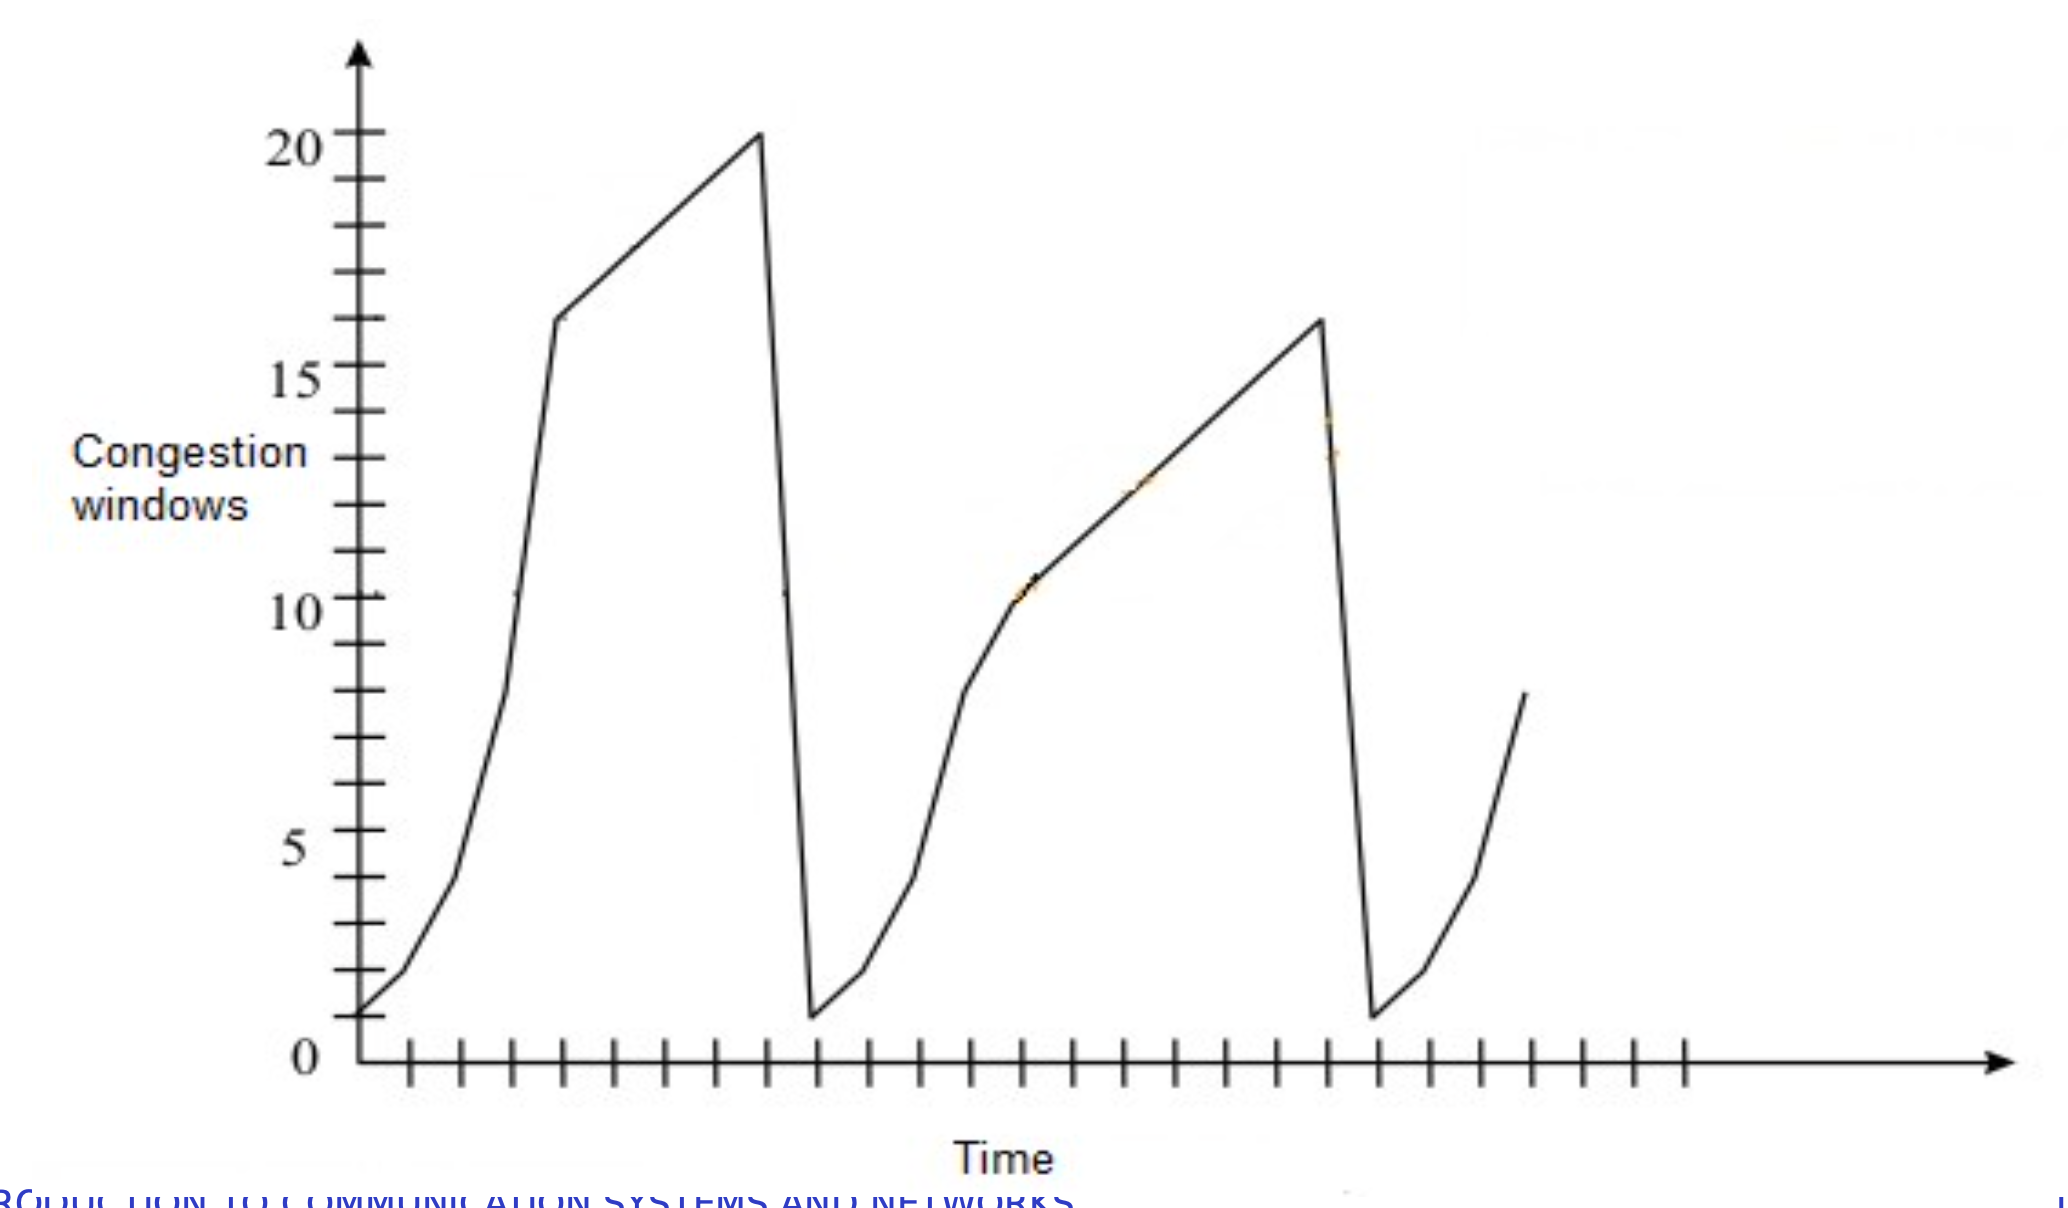
\includegraphics[width=\textwidth]{subfiles/images/part3_q19_window_graphic.png}
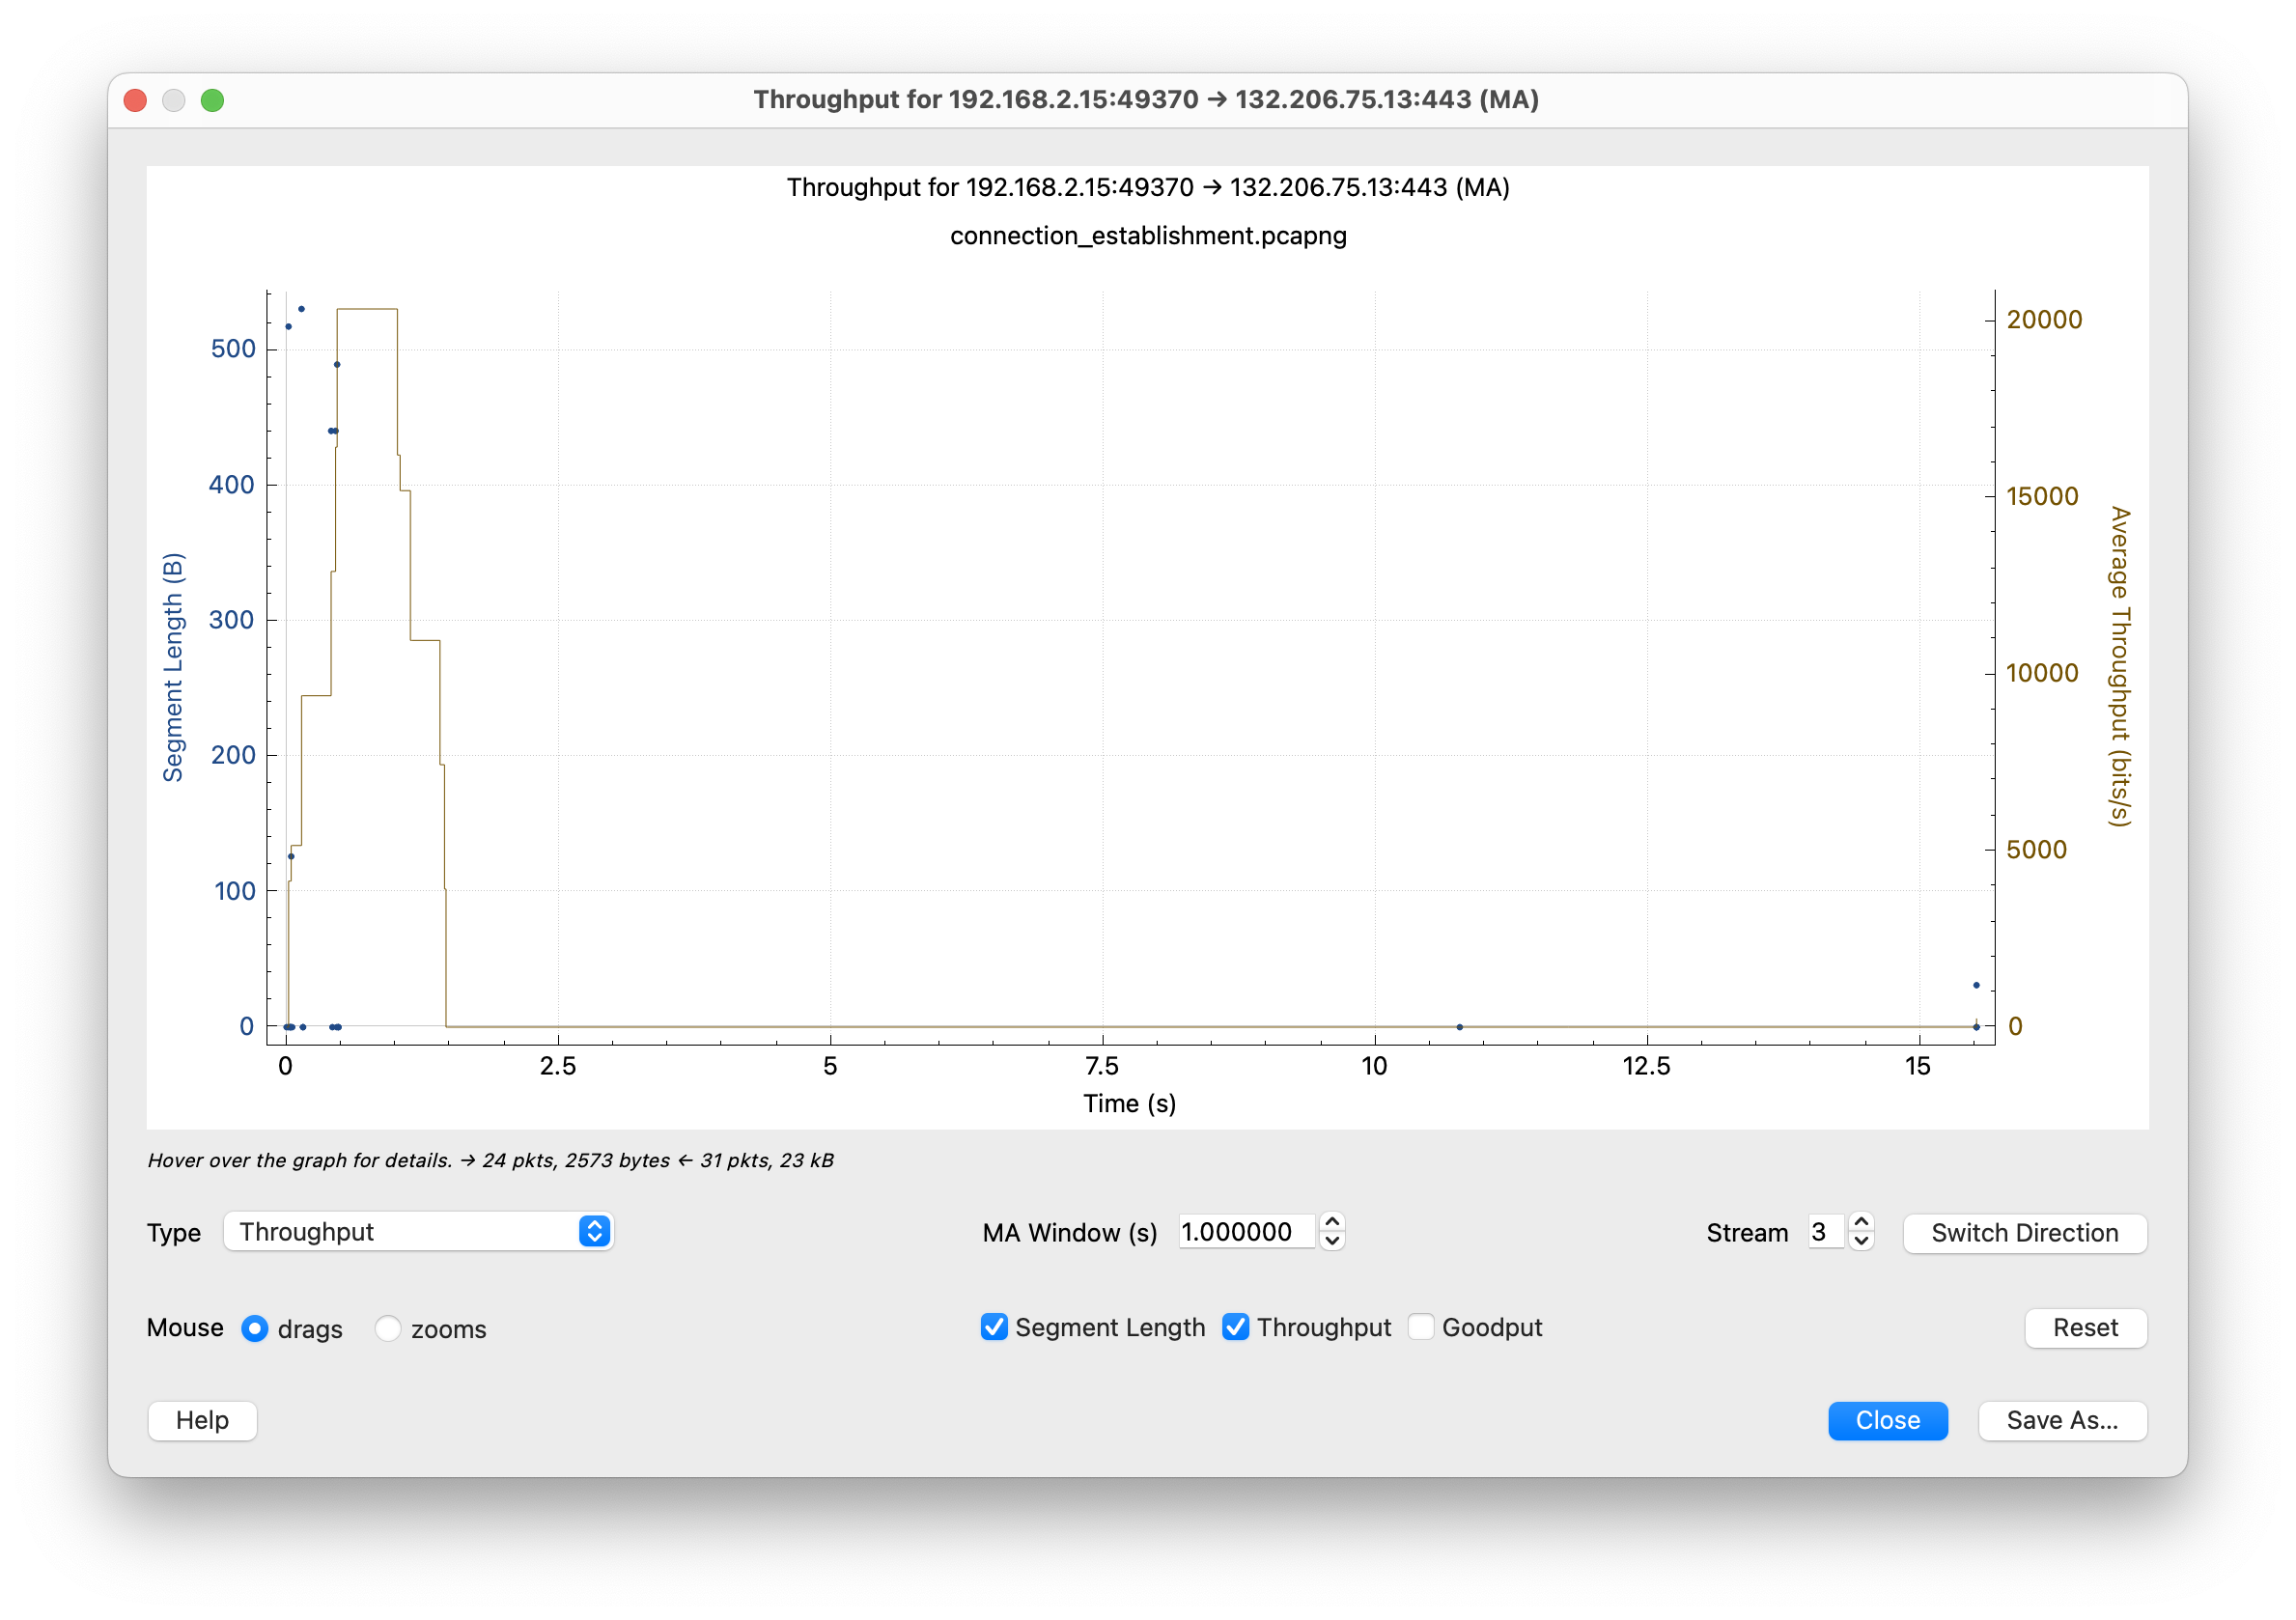
\includegraphics[width=\textwidth]{subfiles/images/throughput_Q15_client_to_server.png}
\end{proof}
\begin{proof}[Proof of Part A]
    Suppose that $S$ is closed, then $\mathbb{Q}$ would be open, and $0\in\mathbb{Q}$ implies that there exists some open $\varepsilon$ ball $V_\varepsilon(0)\subseteq\mathbb{Q}$. \\
    
    Clearly this is absurd, since all open balls in $\real$ are uncountable, and if $V_\varepsilon(0)\subseteq\mathbb{Q}$, it would imply that the open segment $(-\varepsilon,+\varepsilon)$ would be countable, which would in turn mean that $\real$ is countable, since there exists a bijection between $\real$ and any $V_\varepsilon(0)$ if we take
    \[
        f:\real\to V_\varepsilon(0),\quad x\mapsto \varepsilon(x/(1+|x|))
    \]
    Therefore $S$ is not closed.
\end{proof}

\begin{proof}[Proof of Part B]
    Show that $S$ is open, we can separate this into two cases, suppose that both $x,\,y>0$, and let $r = \min\{|x|,|y|\}/2$. For every $(a,b)\in V_r(x,y)$ we have
    \begin{align*}
        (a,b)\in V_r(x,y)&\iff |a-x|^2+|b-y|^2<r^2\\
        &\iff \begin{cases}|a-x|^2<r^2\\
        |b-y|^2<r^2\end{cases}\\
        &\iff \begin{cases}-r<a-x<r\\
            -r<b-y<r\end{cases}\\
        &\iff \begin{cases}x-r<a\\
            y-r<b\end{cases}\\
        &\iff \begin{cases}0<|x|/2<a\\
            0<|y|/2<b\end{cases}\\
        &\implies ab>0
    \end{align*}
    Conversely, suppose that $x,y<0$, then 
    \begin{align*}
        (a,b)\in V_r(x,y)&\iff |a-x|^2+|b-y|^2<r^2\\
        &\iff \begin{cases}|a-x|^2<r^2\\
        |b-y|^2<r^2\end{cases}\\
        &\iff \begin{cases}-r<a-x<r\\
            -r<b-y<r\end{cases}\\
        &\iff \begin{cases}a<|x|/2+x\\
            y-r<b\end{cases}\\
        &\iff \begin{cases}a<-x/2<0\\
            b<-y/2<0\end{cases}\\
        &\implies ab<0
    \end{align*}
    Therefore, for every $(x,y)\in S$, there exists some $r>0$ where
    \[V_r(x,y)\subseteq S\]
\end{proof}

\begin{proof}[Proof of Part C]
    No, $AB$ is not necessarily open. Set $A=\real$, and $B=\{0\}$, clearly $AB=B$, and $B$ is not open.
\end{proof}
\end{document}